\chapter{Runoff concentration} \label{chap:runConc}
\renewcommand{\tabdir}{chapters/part_processes/runoffConcentration/tab}
\renewcommand{\figdir}{chapters/part_processes/runoffConcentration/fig}

\section{Introduction} \label{sec:runConc_intro}

The term \emph{runoff concentration} describes the transport of the locally generated runoff (see \chapref{chap:runGen}) to the catchment's outlet or the nearest river. In general, the description of water transport covers the phenomena of translation and retention.


%%%%%%%%%%%%%%%%%%%%%%%%%%%%%%%%%%%%%%%%%%%%%%%%%%%%%%%%%%%%%%%%%%%%%%%%%%%%%%%%
%%%%%%%%%%%%%%%%%%%%%%%%%%%%%%%%%%%%%%%%%%%%%%%%%%%%%%%%%%%%%%%%%%%%%%%%%%%%%%%%
%%%%%%%%%%%%%%%%%%%%%%%%%%%%%%%%%%%%%%%%%%%%%%%%%%%%%%%%%%%%%%%%%%%%%%%%%%%%%%%%

\section{Parallel storage model} \label{sec:runConcParStor}

%%%%%%%%%%%%%%%%%%%%%%%%%%%%%%%%%%%%%%%%%%%%%%%%%%%%%%%%%%%%%%%%%%%%%%%%%%%%%%%%

\subsection{Processes and equations} \label{sec:runConcParStor_processes}

In the parallel storage model, it is assumed that runoff concentration can be computed separately for the individual runoff components. For each component, translation and retention is simulated by means of a simple reservoir model. The cumulated runoff from the parallel reservoirs finally represents the sub-basins total runoff (\figref{fig:runConcParStor_scheme}).

\begin{figure}
  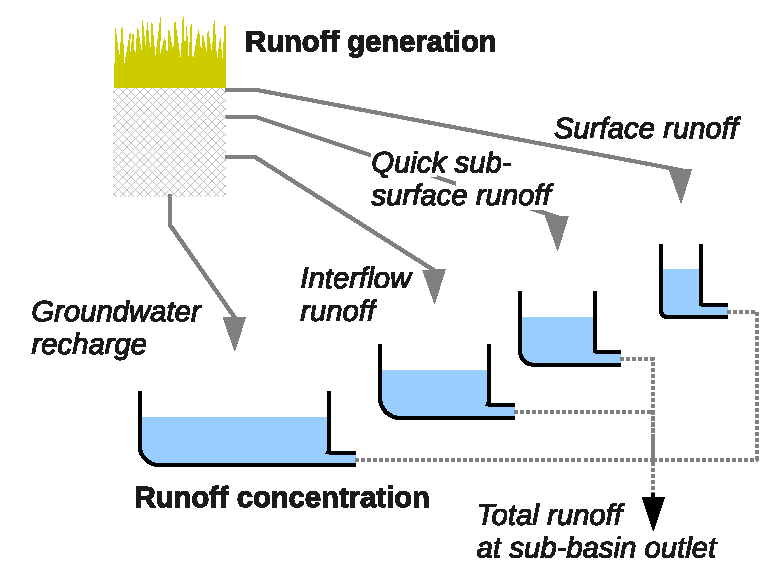
\includegraphics[width=0.9\columnwidth]{\figdir/parallelStorage.eps}
  \caption{Parallel storage model for the case of four runoff components. \label{fig:runConcParStor_scheme}}
\end{figure}

Following the approach used in LARSIM \citep{Ludwig2006}, all reservoirs depicted in \figref{fig:runConcParStor_scheme} are of the linear type. Thus, in addition to the mass balance (\eqnref{eqn:runConcParStor_linResBalance}), the linear relation of \eqnref{eqn:runConcParStor_linResOutflow} applies to each reservoir.

\begin{equation} \label{eqn:runConcParStor_linResBalance}
  \frac{dv}{dt} = q_{in} - q_{out}
\end{equation}
\medskip
\begin{tabular}{lll}
  $v$ & Storage volume & L$^3$ \\
  $q_{in}$ & Inflow rate & L$^3$/T\\
  $q_{out}$ & Outflow rate & L$^3$/T\\
\end{tabular}

\begin{equation} \label{eqn:runConcParStor_linResOutflow}
  q_{out}= \frac{1}{k} \cdot v
\end{equation}
\medskip
\begin{tabular}{lll}
  $k$ & Retention constant & T \\
\end{tabular}

\eqnsref{eqn:runConcParStor_linResBalance} and \ref{eqn:runConcParStor_linResOutflow} can be combined and integrated over time using the substitution method. Assuming that the inflow rate $q_{in}$ is constant over a discrete time step, the integration yields \eqnref{eqn:runConcParStor_linResSolution} as the solution for the storage volume.

\begin{equation} \label{eqn:runConcParStor_linResSolution}
  v(t_0 + \Delta t) =  (v(t_0) - q_{in} \cdot k) \cdot e^{(-\Delta t / k)} + q_{in} \cdot k
\end{equation}
\medskip
\begin{tabular}{lll}
  $v(t_0)$ & Initial storage at & L$^3$ \\
  $\Delta t$ & Length of time step & T \\
\end{tabular}

The only parameters in this runoff concentation model are the values of the retention constants $k$ (one for each reservoir shown in \figref{fig:runConcParStor_scheme}. Regarding these constants, we can formulate two expectations:

\begin{enumerate}
  \item Larger values of $k$ result in a higher retention effect and thus in a more delayed input-output reaction (\figref{fig:runConcParStor_singleLinReserv}). Consequently, we expect the highest $k$ value for the groundwater reservoir while the smallest $k$ value corresponds to the reservoir describing the concentration of surface runoff.
  \item Furthermore, it seems legitimate to assume a relation between the $k$ values and the characteristics of a sub-basin. In particular, we expect smaller retention constants in regions with steep hill slopes, dense drainage networks, and for sub-basin of compact shape.
\end{enumerate}

\begin{figure}
  \includegraphics[width=0.9\columnwidth,angle=270]{\figdir/singleLinearReservoir.eps}
  \caption{Outflow hydrographs from a single linear reservoir for an identical input signal but different storage constants $k$ (hours). \label{fig:runConcParStor_singleLinReserv}}
\end{figure}

To take these two aspect into account, it is convenient to define the retention constants as in \eqnsref{eqn:runConcParStor_retConstSurf} to \ref{eqn:runConcParStor_retConstBase}.

\begin{align}
\text{Surface runoff:} && k = \strSurf \cdot \concTimeIndex \label{eqn:runConcParStor_retConstSurf} \\
\text{Preferential flow:} && k = \strPref \cdot \concTimeIndex \label{eqn:runConcParStor_retConstPref} \\
\text{Interflow:} && k = \strInter \cdot \concTimeIndex \label{eqn:runConcParStor_retConstInter} \\
\text{Base flow:} && k = \strBase \cdot \concTimeIndex \label{eqn:runConcParStor_retConstBase}
\end{align}

Here, \strSurf, \strPref, \strInter, and \strBase{} are dimensionless calibration parameters, fulfilling $\strSurf < \strPref < \strInter < \strBase$ (recall \first{} point of above enumeration). Furthermore, \concTimeIndex{} is an indicator of the sub-basin's runoff concentration characteristics having the dimension of a time (\second{} point of above enumeration). For estimating the \concTimeIndex{} different approaches do exist. In LARSIM \citep{Ludwig2006}, for example, an empirical formula derived by \citet{Kirpich1940} is used. This one computes the \concTimeIndex{} from the average length and slope of the major reach(es) in a sub-basin. Alternatively, a \concTimeIndex{} can be derived by analysis of a digital elevation model. This approach is described in the documentation of the \software{topocatch} preprocessor \citep[see][]{Echse-Tools-Doc}.

See \secref{sec:runConcParStor_hints} for the relation between the $k$ values and the half-life time \halflife{}.

The inflow rate $q_{in}$ (\cbm/s) appearing in \eqnsref{eqn:runConcParStor_linResBalance} to \ref{eqn:runConcParStor_linResSolution} is generally obtained by multiplying the runoff rate (m/s) by the contributing area (\sqm). For the reservoir describing the concentration of surface runoff, $q_{in}$ is usually composed of the runoff generated on saturated soils, water surfaces, and also impervious surfaces.

%%%%%%%%%%%%%%%%%%%%%%%%%%%%%%%%%%%%%%%%%%%%%%%%%%%%%%%%%%%%%%%%%%%%%%%%%%%%%%%%

\subsection{Mathematical solution} \label{sec:runConcParStor_solution}

In each time step, the storage of the four reservoirs is updated based on \eqnref{eqn:runConcParStor_linResSolution} using the individual inflow rates and retention constants (\eqnsref{eqn:runConcParStor_retConstSurf} to \ref{eqn:runConcParStor_retConstBase}). The total outflow from a sub-basin is then obtained as the sum of the outflow rates from the four linear reservoirs.

Note that, if \eqnref{eqn:runConcParStor_linResOutflow} is applied to the already updated storage volumes, the computed outflow rates are \emph{instantaneous values} which correspond to the \emph{end} of a time step. To ensure conservation of mass, these rates should not be directly used as inputs for a downstream model (usually a flow routing model). Instead, \emph{time-step averaged} outflow rates must be passed to the downstream model. For each reservoir, the time-step averaged outflow rates are obtained from the discrete version of the mass balance equation (recall \eqnref{eqn:runConcParStor_linResBalance}) as shown in \eqnref{eqn:runConcParStor_averageOutflow}.

\begin{equation} \label{eqn:runConcParStor_averageOutflow}
  \overline{q_{out}} = q_{in} - \frac{v(t_0 + \Delta t) - v(t_0)}{\Delta t}
\end{equation}
\medskip
\begin{tabular}{lll}
  $\overline{q_{out}}$ & Time-step averaged outflow rate & L$^3$/T\\
  $q_{in}$ & Inflow rate (constant over $\Delta t$) & L$^3$/T \\
  $v(t_0)$ & Initial storage volume & L$^3$ \\
  $v(t_0 + \Delta t)$ & Storage at end of time step & L$^3$ \\
\end{tabular}

%%%%%%%%%%%%%%%%%%%%%%%%%%%%%%%%%%%%%%%%%%%%%%%%%%%%%%%%%%%%%%%%%%%%%%%%%%%%%%%%

\subsection{Implementation} \label{sec:runConcParStor_implementation}

\tabref{tab:runConcParStor_implementation} relates the identifier names used in the model implementation (names of state variables and parameters) to the symbols used in the process equations (\secref{sec:runConcParStor_processes}).

\begin{table*}
\caption{Symbols used in the process equations (\secref{sec:runConcParStor_processes}) and  corresponding identifiers. \label{tab:runConcParStor_implementation}}
\begin{tabular}{|p{0.2\textwidth}p{0.13\textwidth}p{0.07\textwidth}p{0.42\textwidth}|}  \hline
\rowcolor[gray]{0.9}
Symbol & Identifier & Units & Details \\ \hline
$v$ (surface runoff) & \verb!vol_surf! & \cbm{} & Storage volume of surface runoff reservoir \\
$v$ (preferential flow) & \verb!vol_pref! & \cbm{} & Storage volume of preferential flow reservoir \\
$v$ (interflow) & \verb!vol_inter! & \cbm{} & Storage volume of interflow reservoir \\
$v$ (baseflow) & \verb!vol_base! & \cbm{} & Storage volume of baseflow reservoir \\
\strSurf & \verb!str_surf! & sec & Retention constant of surface runoff reservoir \\
\strPref & \verb!str_pref! & sec & Retention constant of preferential flow reservoir \\
\strInter & \verb!str_inter! & sec & Retention constant of interflow reservoir \\
\strBase & \verb!str_base! & sec & Retention constant of baseflow reservoir \\ \hline
\end{tabular}
\end{table*}

%%%%%%%%%%%%%%%%%%%%%%%%%%%%%%%%%%%%%%%%%%%%%%%%%%%%%%%%%%%%%%%%%%%%%%%%%%%%%%%%

\subsection{Hints for application} \label{sec:runConcParStor_hints}

As with all state variables, initial values must be assigned to the storage volumes listed in \tabref{tab:runConcParStor_implementation}. These values are generally unknown and cannot be derived from observation data. Therefore, a widely used approach is to simply guess the initial values and to allow for a rather long 'warm-up' period of the model (several years). If boundary condition data are available for a limited period of time only, one should run a sequence of warm-up simulations. Guessed initial values are used only in the first run. In all later runs, the model is initialized with the final state of the previous run. The success of the latter strategy can be checked, for example, by plotting some simulated hydrographs. If the differences between the hydrographs of consecutive runs becomes negligible, the desired equilibrium of the storage volumes has been reached. However, even then, the initial part of a simulated time series should not be compared to observations because the initial state is still a (refined) guess.

The retention constants listed in \tabref{tab:runConcParStor_implementation} need to be identified by calibration. The values depend on the characteristics of the modeled basin, the model's resolution, as well as on the definition of the used concentraction time index, \concTimeIndex{} (see \eqnsref{eqn:runConcParStor_retConstSurf} to \ref{eqn:runConcParStor_retConstBase}). When calibrating the retention constants, one should keep in mind that a particular parameter set is reasonable only if $\strSurf < \strPref < \strInter < \strBase$ (see \secref{sec:runConcParStor_processes} for details).

The time for model calibration can be reduced (and the overall chance of success can be increased), if prior knowledge on the magnitude of the retention constants is available. If a calibrated model for another nearby basin is available, one could try to adopt the values used in this model as initial guesses. However, this will only work if the basins' characteristics in terms of climate, geomorphology, and land-use are really comparable. Furthermore, the two models must also be comparable with respect to the spatial and temporal discretization.

If another model for a nearby basin is not available or the mentioned conditions are not met, one can try to infer estimates of the retention constants from observed discharge hydrographs. For that purpose, one has to analyze the shape of stream flow recessions using the theory of the single linear reservoir.

Substituting the volume $v$ in \eqnref{eqn:runConcParStor_linResSolution} using \eqnref{eqn:runConcParStor_linResOutflow} yields an equation to predict the future outflow of a linear reservoir using a known initial outflow rate (\eqnref{eqn:runConcParStor_linResSolution_flow}).

\begin{equation} \label{eqn:runConcParStor_linResSolution_flow}
  q_{out}(t_0 + \Delta t) =  (q_{out}(t_0) - q_{in}) \cdot e^{(-\Delta t / k)} + q_{in}
\end{equation}

During recession some time after a flow peak, we can assume that the outflow from the reservoir is much higher than the inflow. Assuming zero inflow, \eqnref{eqn:runConcParStor_linResSolution_flow} simplifies to \eqnref{eqn:runConcParStor_linResSolution_flow_zeroInput}

\begin{equation} \label{eqn:runConcParStor_linResSolution_flow_zeroInput}
  q_{out}(t_0 + \Delta t) =  q_{out}(t_0) \cdot e^{(-\Delta t / k)}
\end{equation}

which can then be solved for the storage constant $k$ (\eqnref{eqn:runConcParStor_kEstim}). Note that all values appearing at the right hand side of this equation are easily obtained from a hydrograph plot (\figref{fig:runConcParStor_recession}).

\begin{equation} \label{eqn:runConcParStor_kEstim}
  k = \frac{\Delta t}{ln(q_{out}(t_0) / q_{out}(t_0 + \Delta t))}
\end{equation}

\begin{figure}
  \centering
  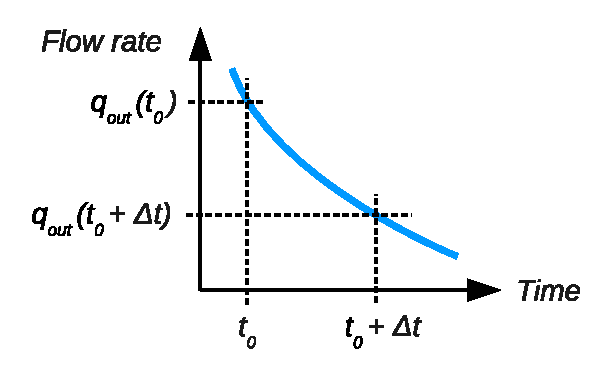
\includegraphics[width=0.75\columnwidth]{\figdir/recession.eps}
  \caption{Analysis of the recession following a flow peak. \label{fig:runConcParStor_recession}}
\end{figure}

When using \eqnref{eqn:runConcParStor_kEstim} to estimate the model parameters \strSurf{}, \strPref{}, \strInter{}, and \strBase{}, one must to take \eqnref{eqn:runConcParStor_retConstSurf}--\ref{eqn:runConcParStor_retConstBase} into account. Thus, the values of $k$ computed from \eqnref{eqn:runConcParStor_kEstim} have to be divided by the concentration time index \concTimeIndex{} in order to obtain the desired values of \strSurf{}, \strPref{}, \strInter{}, and \strBase{}.

In practice, the estimation of the storage constants is complicated by the fact that multiple runoff components contribute to stream flow at the same time. Thus, to estimate the value of a particular constant, one has to consider a recession which is likely to be \emph{dominated} by the corresponding process. For example, \strPref{} and possibly \strSurf{} (and possibly \strInter{}) are likely to control the steep part of the recession after major events. To identify \strBase{}, however, one needs analyze long-lasting recessions, preferably at the end of a rainy season. 

In general, the obtained values for \strSurf{}, \strPref{}, \strInter{}, and \strBase{} should be considered as rough estimates only. It is recommended to refine the estimates during calibration.
